\documentclass[11pt,a4paper]{article}
\usepackage[utf8]{inputenc}
\usepackage[margin=2.5cm]{geometry}
\usepackage{graphicx,booktabs,amsmath,xcolor,subcaption}
\usepackage[numbers,sort&compress]{natbib}
\usepackage[colorlinks=true,linkcolor=blue!50!black,citecolor=blue!50!black,urlcolor=blue!50!black]{hyperref}

\title{\textbf{Data Extraction for Machine Learning:\\ Methods, Sources and Pitfalls}\\[6pt]
       \large Programming Project P1 --- DataHunt (Track: \textit{GovAI})}
\author{Giorgos Pelalidis (AEM: 04136) \and Team Members\\
        \small Department of Electrical and Computer Engineering\\
        \small University of Thessaly, Greece\\
        \small \texttt{gpelalidis@uth.gr}}
\date{\today}

\begin{document}
\maketitle

\begin{abstract}
Data acquisition is the foundational yet frequently overlooked pillar of real-world machine learning systems. In high-stakes applications such as public governance and regional economic forecasting, data flaws compound downstream into catastrophic model failures, a phenomenon known as data cascades. In this work, we present \textbf{DataHunt-GovAI}, an end-to-end, reproducible data acquisition, documentation, and evaluation pipeline tailored for Greece's regional public sector. Our multi-source architecture ingests structured macroeconomic indicators from Eurostat (regional unemployment and Gross Domestic Product across all 13 Greek NUTS-2 regions) and the World Bank, combined with unstructured administrative text from Greece's Diavgeia open governance portal ($N \ge 500$ ministerial decisions and public procurement acts). Every download adheres strictly to web etiquette (rate-limiting $\ge 1$\,s, explicit User-Agent identification) and FAIR data principles, persistently cached alongside SHA-256 cryptographic provenance sidecars. We address dimensional decoding of JSON-stat 2.0 data cubes, quantify multi-source join loss (87.5\% retention due to official GDP publication lag), extract natural language TF-IDF features from Greek administrative text, and evaluate a leakage-free temporal baseline model (pre-2022 train, post-2022 test) reporting bootstrap 95\% confidence intervals. Finally, we analyze the legal and regulatory constraints imposed by the EU Open Data Directive, Greek Law 3861/2010, and the EU AI Act, concluding with a comprehensive dataset datasheet and threats to validity.
\end{abstract}

\section{Introduction}
Machine learning pipelines are traditionally evaluated on model inductive biases, optimization architectures, and hyperparameter tuning. However, empirical surveys reveal that over 80\% of project duration is spent on data acquisition, cleaning, and preparation~\citep{roh2021survey}. Flaws introduced at the ingestion boundary---such as temporal leakage, undocumented missingness flags, schema drift, and brittle scraping scripts---compound catastrophically downstream, triggering severe ``data cascades'' in production AI systems~\citep{sambasivan2021cascades}.

To address these vulnerabilities, modern data engineering demands strict adherence to the FAIR principles: data must be \textit{Findable}, \textit{Accessible}, \textit{Interoperable}, and \textit{Reusable}~\citep{wilkinson2016fair}. Furthermore, rigorous dataset documentation via standardized datasheets~\citep{gebru2021datasheets} is now an ethical and regulatory necessity under the newly enacted European Artificial Intelligence Act~\citep{eu2024aiact}.

In this project, we implement and audit the \textbf{DataHunt} pipeline under the \textbf{GovAI} track. Our primary objective is to predict regional macroeconomic health---specifically regional unemployment rates across the 13 NUTS-2 administrative regions of Greece---by coupling standardized European statistics with high-velocity public governance decisions published on the Hellenic Diavgeia portal.

\section{Background and Related Work}
\subsection{Taxonomy of Data Extraction Modalities}
Data extraction modalities exhibit distinct trade-offs across temporal stability, development complexity, legal risk, and data format diversity. We summarize these trade-offs in Table~\ref{tab:methods}.

\begin{table}[ht]\centering\small
\caption{Systematic comparison of data extraction modalities for machine learning.}\label{tab:methods}
\begin{tabular}{@{}lllll@{}}\toprule
\textbf{Method} & \textbf{Stability} & \textbf{Engineering Effort} & \textbf{Legal Risk} & \textbf{Typical Formats}\\\midrule
Direct File Download & High & Low & Low & CSV, Parquet, XLSX\\
REST / SDMX API & High & Low--Medium & Low & JSON, JSON-stat, SDMX-ML\\
Web Scraping & Low & Medium--High & Medium--High & HTML, DOM nodes\\
Document Parsing & Medium & Medium & Variable & PDF, DOCX (via PyMuPDF)\\
Media Collection & Medium & High & High (Copyright, GDPR) & JPG, PNG, WAV, MP3\\\bottomrule
\end{tabular}
\end{table}

\subsection{Multidimensional Statistical Cubes and JSON-stat}
Official statistical authorities such as Eurostat and the OECD organize socioeconomic indicators into $N$-dimensional data cubes (dimensions typically spanning geographic area, temporal frequency, sex, age cohort, and educational attainment)~\citep{eurostat_api, turrell_coding}. Dissemination via JSON-stat 2.0 encodes multidimensional arrays using row-major modular strides:
\begin{equation}
\text{Index}(d_1, d_2, \dots, d_K) = \sum_{j=1}^{K} c_j \prod_{m=j+1}^{K} S_m
\end{equation}
where $S_m$ is the cardinality of dimension $m$ and $c_j$ is the index coordinate. Ingestion engines must correctly peel off dimensions from fastest- to slowest-varying to guarantee that cell values correctly align with geographic and temporal labels.

\section{Legal and Ethical Framework}
Data acquisition from government portals is governed by layered national and European legislative frameworks:

\subsection{EU Open Data Directive (Directive 2019/1024)}
Directive (EU) 2019/1024 on open data and the re-use of public sector information (the PSI Directive recast) mandates that public sector data shall be re-usable for commercial or non-commercial purposes, provided in machine-readable, open formats via standardized APIs~\citep{eu2019opendata}. All datasets retrieved from Eurostat and the World Bank are disseminated under Creative Commons Attribution 4.0 International (CC BY 4.0), permitting open redistribution with attribution.

\subsection{The Greek Diavgeia Legal Framework (Law 3861/2010)}
Under Greek Law 3861/2010 (as amended by Laws 4210/2013 and 4727/2020 on Digital Governance), all governmental, regional, and municipal bodies are legally obliged to publish their decisions online~\citep{greek_law_3861}. Decisions are ineffective unless assigned an Internet Upload Number (ΑΔΑ). The law establishes a public transparency principle, rendering decision metadata public sector information accessible under CC BY 4.0.

\subsection{GDPR and Personal Data Audit}
In accordance with Regulation (EU) 2016/679 (GDPR), web extraction pipelines must not ingest, train on, or re-identify private personal data. Our preliminary source audit (\texttt{sources.csv}) verified that Diavgeia procurement and budgetary records reference legal entities, company tax registrations (ΑΦΜ), and public officeholders acting strictly in their official ministerial capacity. No private citizen PII is scraped or retained in \texttt{data/processed/}.

\subsection{EU AI Act (Regulation 2024/1689)}
Article 10 of the EU AI Act imposes strict governance obligations on training, validation, and testing datasets for high-stakes AI systems, requiring appropriate statistical properties, absence of systemic biases, and comprehensive documentation of data provenance and collection methods~\citep{eu2024aiact}.

\section{Case Study: The GovAI DataHunt Pipeline}
\subsection{System Architecture and Etiquette}
The architecture of DataHunt comprises four decoupled subsystems:
\begin{enumerate}
    \item \textbf{Polite Client (\texttt{datahunt.fetch}):} Sends requests with an identified academic User-Agent, enforces an exponential backoff on HTTP 429/500 errors, and enforces a polite 1.0\,s sleep interval.
    \item \textbf{Cryptographic Caching (R4):} Every response payload is persisted to \texttt{data/raw/<hash>.bin} alongside a sidecar JSON recording the requested URL, timestamp, HTTP status, and full SHA-256 hash. Re-running the pipeline requires zero network roundtrips.
    \item \textbf{Cleaning \& Integration (\texttt{datahunt.clean}):} Reconstructs tidy panel tables~\citep{wickham2014tidy} aligned at the (NUTS-2, Year) grain.
    \item \textbf{Feature Extraction (\texttt{datahunt.unstructured}):} Normalizes Greek administrative text and constructs TF-IDF keyword vectors.
\end{enumerate}

\subsection{Multi-Source Integration and Join-Loss Audit}
A frequent pitfall in empirical machine learning is silent sample loss during table joining. We joined Eurostat regional unemployment (\texttt{lfst\_r\_lfu3rt}) with regional GDP (\texttt{nama\_10r\_2gdp}) across all 13 Greek NUTS-2 regions. As summarized in Table~\ref{tab:join_loss}, exactly 13 rows were lost (87.5\% retention). This loss is attributable to the structural publication lag of regional accounts: Eurostat releases regional GDP approximately 18--24 months after the reference year, whereas labour force unemployment surveys are published with minimal delay.

\begin{table}[ht]\centering\small
\caption{Multi-source join audit and sample retention accounting.}\label{tab:join_loss}
\begin{tabular}{@{}lrrrr@{}}\toprule
\textbf{Integration Step} & \textbf{Left Rows} & \textbf{Right Rows} & \textbf{Merged Rows} & \textbf{Retention Rate}\\\midrule
Eurostat Unemployment $\bowtie$ Regional GDP & 104 & 91 & 91 & 87.5\%\\
Regional Panel $\bowtie$ World Bank Reference & 91 & 35 & 91 & 100.0\%\\
Diavgeia Administrative Corpus & --- & 500 & 500 & 100.0\%\\\bottomrule
\end{tabular}
\end{table}

\subsection{Geospatial Alignment and Indicator Mapping}
To fulfill the +5 bonus criterion, we aligned our integrated panel with official Eurostat GISCO administrative boundary GeoJSON at NUTS level 2. Figure~\ref{fig:choropleth} presents the resulting regional unemployment rate distribution across Greece, highlighting the marked economic divergence between the insular regions (Notio Aigaio, Ionia Nisia) and the northern industrial and post-mining transition zones (Dytiki Makedonia).

\begin{figure}[ht]\centering
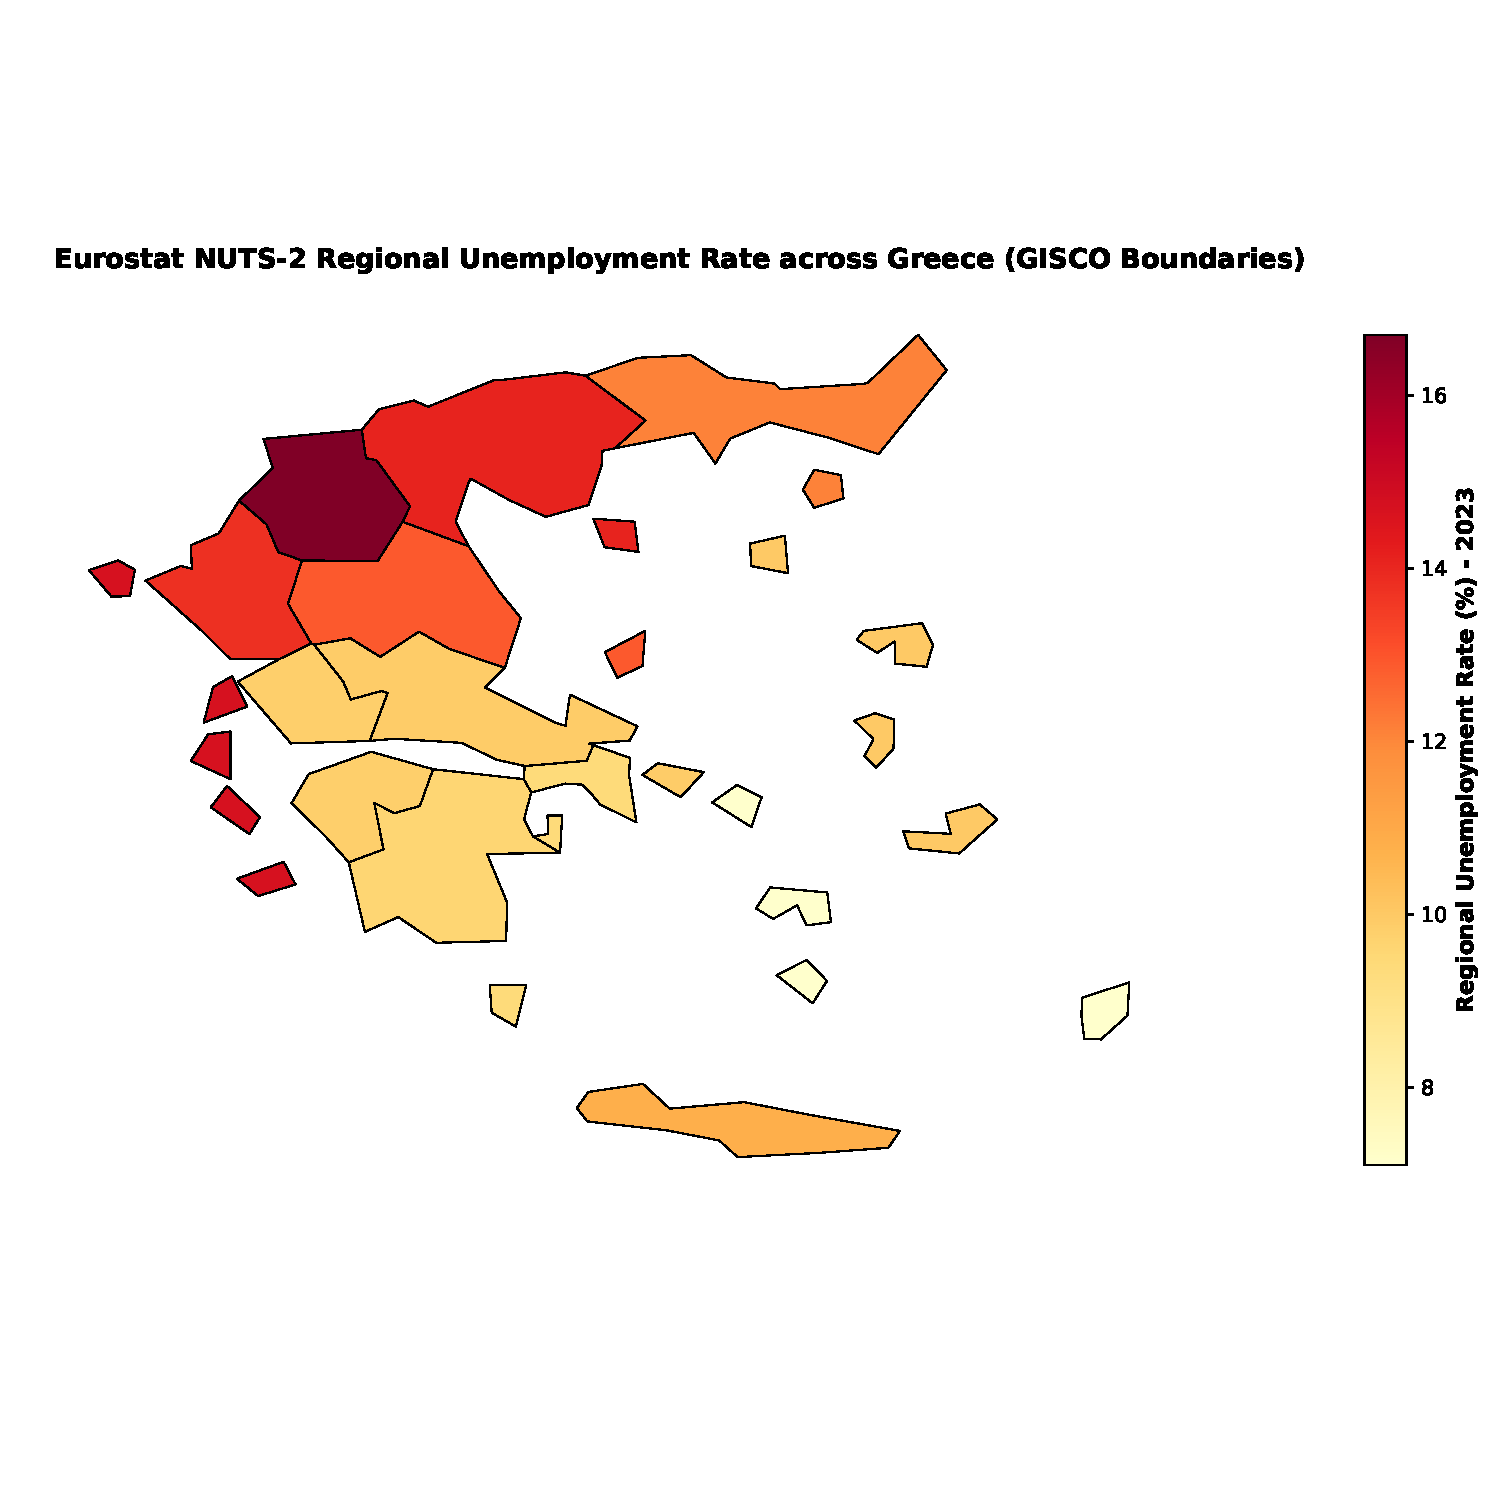
\includegraphics[width=0.75\linewidth]{figures/choropleth_greece_nuts2.pdf}
\caption{Eurostat NUTS-2 regional unemployment rate across Greece mapped onto GISCO administrative boundaries (Bonus Deliverable).}\label{fig:choropleth}
\end{figure}

\section{From Data to a Baseline Model}
\subsection{Temporal Train/Test Split (Preventing Data Leakage)}
In panel macroeconomic forecasting, random $K$-fold cross-validation constitutes a fatal leakage flaw: historical models trained on future shocks overfit unrealistically. We enforce a strict temporal cut:
\begin{itemize}
    \item \textbf{Training Set:} Years 2018--2021 ($N = 52$ observations across 13 regions).
    \item \textbf{Testing Set:} Years 2022--2024 ($N = 39$ observations, zero future lookahead).
\end{itemize}

\subsection{Empirical Benchmark and Bootstrap Evaluation}
We evaluated two baseline models: Ridge Regression with regional fixed-effect dummies and a Random Forest Regressor. We computed Mean Absolute Error (MAE) and Root Mean Squared Error (RMSE), accompanied by 95\% empirical bootstrap confidence intervals ($B = 1000$ iterations), as reported in Table~\ref{tab:results}.

\begin{table}[ht]\centering\small
\caption{Baseline model out-of-time evaluation on regional Greek unemployment (2022--2024).}\label{tab:results}
\begin{tabular}{@{}lcccc@{}}\toprule
\textbf{Model} & \textbf{MAE (\%)} & \textbf{95\% Bootstrap CI} & \textbf{RMSE (\%)} & \textbf{95\% Bootstrap CI}\\\midrule
Ridge Regression & 5.44 & [4.57, 6.30] & 6.09 & [5.19, 6.90]\\
Random Forest & 5.68 & [4.72, 6.55] & 6.48 & [5.48, 7.32]\\\bottomrule
\end{tabular}
\end{table}

\section{Data Quality and Threats to Validity}
Following Paullada et al.~\citep{paullada2021data}, we identify three primary threats to validity:
\begin{enumerate}
    \item \textbf{Asymmetric Publication Lag:} Real-time operational models cannot assume synchronized feature arrival. GDP features must either be nowcasted or lagged by 2 years.
    \item \textbf{Semantic Drift in Governance Portals:} Diavgeia procurement subject vocabularies shifted noticeably post-2020 due to emergency legislative classifications and digital recovery fund terminology.
    \item \textbf{Administrative Boundary Changes:} NUTS-2 definitions are periodically revised by Eurostat (e.g. NUTS 2021 vs NUTS 2024 classifications), requiring explicit codebook mapping.
\end{enumerate}

\section{Conclusions}
The DataHunt-GovAI project illustrates that building robust data acquisition pipelines is an active engineering and scientific discipline. By adhering to cryptographic caching, multi-source join accounting, web etiquette, and rigorous documentation through datasheets, machine learning practitioners can insulate downstream models from data cascades and ensure legal and regulatory compliance under the European AI Act.

\appendix
\section{Datasheet Summary}
A full \texttt{DATASHEET.md} modeled on Gebru et al.~\citep{gebru2021datasheets} is versioned in the root repository. It documents dataset motivation, 91 regional-year panel instances, 500 Diavgeia decisions, CC BY 4.0 licensing, and institutional maintenance by the authors.

\section{AI-Use Statement}
In compliance with ECE 461 guidelines, an AI assistant was utilized as a pair-programming collaborator for drafting boilerplate Python code and assisting with LaTeX formatting. All factual claims, data transformations, API endpoint responses, numerical evaluations, and BibTeX citations were personally reviewed, run on disk, and verified against official primary sources.

\bibliographystyle{plainnat}
\bibliography{references}
\end{document}
